\documentclass[12pt, openany]{book}
\usepackage{algorithm2e}

% This is all the packages and settings and so on.
% It is using custom fonts that needs to be installed on the computer. If they are not present, they have to be added manually.
\usepackage[
	citestyle=ieee, 
    bibstyle=ieee,
    style=numeric-comp,
    sorting=nty,
    maxbibnames=99, % Make sure we are printing all authors in the appendix
    ]{biblatex}
    
% Makes the last name first in the bibliography.
% \DeclareNameAlias{author}{last-first}
\DeclareNameAlias{author}{family-given}
    
% Specify the margins. This is 6.25inches in text with which 
% can be used to size figures to the correct size.
\usepackage[a4paper, margin=2.5625cm]{geometry}

\usepackage{eso-pic}					% Packages for layout and graphics 
\usepackage{graphicx}
\usepackage{tikz}
\usetikzlibrary{fadings}
\usepackage{setspace}
% \usepackage{tocloft}		 			% Fixing a bug with page style changes for toc
% \tocloftpagestyle{plain}
\usepackage{etoc} 						% Separate tocs for appendix and the rest    
\usepackage{chngcntr}					% Count figures within chapters
\usepackage{booktabs}					% Table formatting
\usepackage{fancyhdr}					% Setting the style for header and footer.
\usepackage{tabularx}
\usepackage{multirow}                   % For better tables 
\usepackage[hidelinks]{hyperref}		% Clickable links
\usepackage{nameref}					% References with names
\usepackage[parfill]{parskip}			% New line instead of indent for sections
\usepackage{tcolorbox}					% Create boxes around content
\tcbset{colback=white,arc=0mm}

\usepackage{amsmath}
\usepackage{mathdots}
\usepackage{yhmath}
\usepackage{siunitx}
\usepackage{array}
\usepackage{gensymb}
\usepackage{amssymb}
\usepackage{mathtools}              % Add text to math arrows.

\usepackage{cancel}
\usepackage{color}
\usepackage{multirow}
\usepackage{textcomp}               % Fixing warning for gensyb \perthousand
\usepackage{svg}                    % including svg files
\usepackage{caption}                % For subfigures
\usepackage{subcaption}
\usepackage{fontspec}
\usepackage{sectsty}
\usepackage{tocloft}

\usepackage[printonlyused]{acronym}


\counterwithin{figure}{section} 
\counterwithin{table}{section}

% Specifying fonts
\setmainfont{Georgia} 
\setsansfont{Arial}
\newfontfamily\footerfont{Georgia}

\chapterfont{\sffamily\fontsize{17}{17}}
\sectionfont{\sffamily\fontsize{14}{15}}
\subsectionfont{\sffamily\fontsize{13}{15}}
\subsubsectionfont{\sffamily\fontsize{12}{15}}

% Remove the title and make sure that the text is adjusted
% \usepackage{abstract}
% \setlength{\absleftindent}{0mm}
% \renewcommand{\abstractname}{\vspace{-\baselineskip}}
% \renewcommand{\abstractnamefont}{\sffamily\fontsize{14}{15}}
% \renewcommand{\abstracttextfont}{\normalfont\fontsize{12}{13}}

% Renaming and setting style of table of contents
\renewcommand*\contentsname{Contents}
\renewcommand*\cfttoctitlefont{\fontsize{16}{0}\bf\sffamily}
\renewcommand\cftchapfont{\fontsize{14}{0}\bf\sffamily}
\renewcommand\cftchappagefont{\fontsize{13}{0}\bf\sffamily}
\renewcommand\cftsecfont{\fontsize{12}{0}\sffamily}
\renewcommand\cftsecpagefont{\fontsize{12}{0}\sffamily}
\renewcommand\cftsubsecfont{\fontsize{12}{0}\sffamily}
\renewcommand\cftsubsecpagefont{\fontsize{12}{0}\sffamily}

% Styling the header and footer
\fancyhf{}
\fancyhead{}
\fancyfoot{}
\fancyhead[L]{\fontsize{11}{10}\selectfont\leftmark}
\fancyfoot[R]{\footerfont\thepage}
\setlength{\headheight}{15.5pt}


\fancypagestyle{plain}{
    \fancyhf{}
    \fancyhead{}
    \fancyfoot{}
    \renewcommand{\headrulewidth}{0pt}
    \fancyfoot[R]{\footerfont\thepage}
}

\pagestyle{fancy}

% Making the command for placing text in random locations
\newcommand\PlaceText[3]{%
\begin{tikzpicture}[remember picture,overlay]
\node[outer sep=0pt,inner sep=0pt,anchor=south west] 
  at ([xshift=#1,yshift=-#2]current page.north west) {#3};
\end{tikzpicture}%
}

% Disable hyphenation
\pretolerance=10000
\tolerance=2000 
\emergencystretch=50pt


% Defining files for bibliography
%\addbibresource{ref.bib}
\addbibresource{/Users/xinyi/Documents/GitHub/mythesis/references.bib}

% Add a second bibliography file for the second author to allow
% both to update it through the mendeley integration.
% \addbibresource{ref-author-2.bib}

% Defining document information
\title{Assessing the Streamline Plausibility Through \textit{Convex Optimization for Microstructure Informed Tractography}(COMMIT) with Deep Learning}
\newcommand{\subtitle}{KTH Thesis Report}
\author{Xinyi Wan}

\begin{document}
\setstretch{1.4}

% The front page of the document
\pagenumbering{roman}
\makeatletter
\begin{titlepage}

\vspace*{-4.6\baselineskip}
\hspace*{-0.15\textwidth}
\includegraphics[width=0.2\paperwidth]{setup/img/kth-logo.jpg}
\par\vspace*{2.5\baselineskip}

\PlaceText{65mm}{12mm}{\fontsize{12}{0}\sffamily DEGREE PROJECT IN TECHNOLOGY,}
\PlaceText{65mm}{17mm}{\fontsize{12}{0}\sffamily SECOND CYCLE, 30 CREDITS}
\PlaceText{65mm}{22mm}{\fontsize{12}{0}\sffamily\itshape STOCKHOLM, SWEDEN \the\year}

~\\

\makebox[0pt][l]{%
\begin{minipage}[b]{0.25\textwidth}
~\\
\end{minipage}
\begin{minipage}{0.65\textwidth}
\begin{flushleft}
{\fontsize{28}{24}\bf\sffamily\@title\\}
\vspace{1cm}
{\fontsize{19}{17}\bf\sffamily \subtitle\\}
\vspace{1cm} 
{\fontsize{16}{18}\sffamily \@author}\\
\end{flushleft}
\end{minipage}
}


% \hspace*{-3cm}\begin{minipage}[b]{63.5mm}
% ~\\
% \end{minipage}
% \begin{minipage}{0.65\textwidth}
% \begin{flushleft}
% {\fontsize{28}{24}\bf\sffamily\@title\\}
% \vspace{0.5cm}
% {\fontsize{19}{17}\bf\sffamily \subtitle\\}
% \vspace{0.5cm} 
% {\fontsize{16}{0}\sffamily \@author}\\
% \end{flushleft}
% \end{minipage}


\AddToShipoutPictureBG*{%]
    \AtPageLowerLeft{%
        
\includegraphics[width=1.0\paperwidth]{setup/img/kth-footer.png}
    }%
}

\PlaceText{70mm}{280mm}{\color{white}\fontsize{12}{0}\sffamily KTH ROYAL INSTITUTE OF TECHNOLOGY }
\PlaceText{70mm}{285mm}{\color{white}\fontsize{8}{0}\sffamily ELECTRICAL ENGINEERING AND COMPUTER SCIENCE }
\end{titlepage}
\makeatother

\newpage
\newpage
\thispagestyle{plain}
~\\
\vfill
{ \setstretch{1.1}
	\subsection*{Authors}
	Xinyi Wan <xinyiwan@kth.se>\\
	School of Engineering Sciences in Chemistry, Biotechnology and Health\\
	KTH Royal Institute of Technology
	
	\subsection*{Place for Project}
	Division of Biomedical Imaging\\
	KTH Royal Institute of Technology
	
	\subsection*{Examiner}
	Matilda Larsson\\
	HÄLSOVÄGEN 11 C, HUDDINGE \\
	KTH Royal Institute of Technology
	
	\subsection*{Supervisor}
	Rodrigo Moreno\\
	HÄLSOVÄGEN 11 C, HUDDINGE\\
	KTH Royal Institute of Technology

	\subsection*{Swedish title}
	Bedömning av strömlinjeformligheten genom\\
	konvex optimering för mikrostrukturinformerad \\
	traktografi (COMMIT) med djupinlärning
	~
}


\newpage
\thispagestyle{plain}
%%%%%%%%%%%%%%%%%%%%%%%%%%%%%%%%%%%%
%%  The English abstract          %%
%%%%%%%%%%%%%%%%%%%%%%%%%%%%%%%%%%%%
\chapter*{Abstract}
%%%%%%%%%%%%%%%%%%%%%%%%%%%%%%%%%%%%

Tractography is widely used in the brain connectivity study from diffusion magnetic resonance imaging data. 
However, lack of ground truth and plenty of 
anatomically implausible streamlines in the tractograms have caused challenges and concerns in the use of tractograms such as brain connectivity study.
Tractogram filtering methods have been developed to remove the faulty connections.
In this study, we focus on one of these filtering methods, \textit{Convex Optimization Modeling for Microstructure Informed Tractography} (COMMIT),
which tries to find a set of streamlines that best reconstruct the diffusion magnetic resonance imaging data with global optimization approach.
There are biases with this method when assessing individual streamlines. 
So a method named randomized COMMIT(rCOMMIT) is proposed to obtain multiple assessments for each streamline.
The acceptance rate from this method is introduced to the streamlines and divides them into three groups, which 
are regarded as pseudo ground truth from rCOMMIT. Therefore, the neural networks are able to train on the pseudo ground truth on 
classification tasks. The trained classifiers distinguish the obtained groups of plausible and implausible streamlines with accuracy around 77\%.
Following the same methodology, the results from rCOMMIT and randomized SIFT are compared. 
The intersections between two methods are analyzed with neural networks as well, which achieve accuracy around 87\% in binary task between plausible and implausible streamlines.



\subsection*{Keywords}
Tractography, dMRI, Filtering Methods, Deep Learning, Classification




\newpage
\thispagestyle{plain}
%%%%%%%%%%%%%%%%%%%%%%%%%%%%%%%%%%%%
%%	 The Swedish abstract         %%
%%%%%%%%%%%%%%%%%%%%%%%%%%%%%%%%%%%%
\chapter*{Sammanfattning}
%%%%%%%%%%%%%%%%%%%%%%%%%%%%%%%%%%%%
Traktografi är ett verktyg och används ofta i hjärnanslutningsstudien från
magnetisk resonansavbildningsdata för diffusion. Dock brist på grundsanning och gott om
anatomiskt osannolika strömlinjer i traktogrammen har orsakat utmaningar och bekymmer.
Traktogramfiltreringsmetoder har utvecklats för att ta bort de felaktiga anslutningarna.
I denna studie fokuserar vi på en av dessa filtreringsmetoder, \textit{Convex Optimization Modeling for Microstructure Informed Tractography} (COMMIT),
som försöker hitta en uppsättning strömlinjer som bäst rekonstruerar diffusionsmagnetisk resonansavbildningsdata med global optimeringsmetod.
Det finns fördomar med denna metod när man bedömer individuella effektiviseringar.
Så en metod som heter randomized COMMIT(rCOMMIT) föreslås för att få flera bedömningar för varje effektivisering.
Acceptansgraden från denna metod introduceras till effektiviseringarna och delar upp dem i tre grupper, som
betraktas som pseudogrund sanning från rCOMMIT. Därför kan de neurala nätverken träna på pseudogrunden sanning på
klassificeringsuppgifter. De tränade klassificerarna särskiljer de erhållna grupperna av rimliga och osannolika strömlinjer med en noggrannhet runt 77\%.
Enligt samma metodik jämförs resultaten från rCOMMIT och randomiserat SIFT.
Skärningspunkterna mellan två metoder analyseras också med neurala nätverk, som uppnår en noggrannhet runt 87\% i binär uppgift mellan rimliga och osannolika strömlinjer.
\subsection*{Nyckelord}
Traktografi, dMRI, filtreringsmetoder, djupinlärning, klassificering

\newpage
\thispagestyle{plain}
\chapter*{Acknowledgements}
I would like to express my sincere gratitude to my supervisor Rodrigo Moreno for his invaluable guidance and support 
throughout my master study. Without his constant encouragement and insightful feedback I would not have been able to complete this project.
Moreover, I would like to thank the PhD students in our research group at KTH, 
Mehdi Astaraki, Fabian Sinzinger, Simone Bendazzoli, Jingru Fu for providing me feedbacks and insights when I struggled with my project.
Many thanks should also go to the master students in our group, Karine Louis, Lasse Stahnke and Yuqi Zheng. 
Our discussions and fika time were not only valuable but also enjoyable.
Finally, I want to express my deepest gratitude to my family for their support and encouragement throughout my academic journey.

\newpage

% \chapter*{Acronyms}


% \begin{acronym}
% \acro{dMRI}{Diffusion Magnetic Resonance Imaging}
% \acro{USA}{United States of America}

% \end{acronym}

\begin{acronym}
    \acro  {iot}   [IoT]   {Internet-of-Things}
    \acro  {icann} [ICANN] {Internet Corporation for Assigned names and Numbers}
    \acro  {iso}   [ISO]   {International Organization for Standardization}
    \acro  {ietf}  [IETF]  {Internet Engineering Task Force}    % will not be listed, as it is no
\end{acronym}


\newpage

\etocdepthtag.toc{mtchapter}
\etocsettagdepth{mtchapter}{subsection}
\etocsettagdepth{mtappendix}{none}
\thispagestyle{plain}
\tableofcontents

\newpage



\chapter*{Acronyms}


% \begin{acronym}
% \acro{dMRI}{Diffusion Magnetic Resonance Imaging}
% \acro{USA}{United States of America}

% \end{acronym}

\begin{acronym}
    \acro  {iot}   [IoT]   {Internet-of-Things}
    \acro  {icann} [ICANN] {Internet Corporation for Assigned names and Numbers}
    \acro  {iso}   [ISO]   {International Organization for Standardization}
    \acro  {ietf}  [IETF]  {Internet Engineering Task Force}    % will not be listed, as it is no
\end{acronym}


\pagenumbering{arabic}

\chapter{Introduction}

Diffusion magnetic resonance imaging(dMRI) is a powerful imaging modality capable of inferring the local axonal structure in each imaging voxel by exploiting the natural random movement of water molecules in biological tissues \cite*{intro}. Tractography is a set of algorithms aiming at mapping the major neuronal pathways in the white matter of the brain from dMRI signals. Based on the estimated direction of neuronal fibres from dMRI data, the tractogram of the brain could be generated with tractography, which consists of numerous streamlines that 
represent the microstructure of brain tissues. 
According to its technical features, the tractography of dMRI could contribute to the noninvasive investigation of brain connectivity and have potential in clinical research. 

However, there are still concerns and challenges with tractography. The anatomically implausible streamlines from the tractography might influence research results from tractogram, such as the analysis of brain connectivity. To solve this problem, tractogram filtering methods have been developed to remove the faulty connections in a post-processing step \cite{hainAssessingStreamlinePlausibility2022a}.
This project mainly analyses one of the tractogram filtering tools, \textit{Convex Optimization Modeling for Microstructure Informed Tractography} (COMMIT), which aims at reestablishing the link between tractography and tissue microstructure \cite{daducciCOMMITConvexOptimization2015}. 
Meanwhile, this project will compare with the results from the study focusing on the performance of another filtering method named \textit{Spherical-deconvolution informed filtering of tractograms} (SIFT) \cite{smithSIFTSphericaldeconvolutionInformed2013}.

First, the project plans to investigate the performance of COMMIT by applying it multiple times to the subsets of the same subject. The results from filtering methods are not always consistent, and might be sensitive to the size and composition of the inputs. For example, a streamline from the same subject can be accepted by the filtering method in one run but rejected in another. Although the anatomical ground truth is absent, a pseudo ground truth could be generalized from the partly consistent results of COMMIT. By applying COMMIT to multiple tractogram subsets, consistent assessments for each streamline are extracted
as pseudo-ground truths. The streamlines that are always accepted by COMMIT will be regarded as true streamlines,
while those which are always rejected will be regarded as false streamlines. And the streamlines with different
results are regarded as inconclusive streamlines.

With these assumptions, deep learning methods are exploited in the second part of this project.
The classifiers based on different deep learning architectures are used to distinguish different groups of streamlines. The potential of using deep learning methods in filtering is the focus of this part of study.

% \chapter{Theoretical Background}


In this chapter, theoretical background of this project will be introduced in details. To better introduce the importance of the filtering, a big picture of the pipeline of tractography will be first presented. 

\section{Diffusion MRI}

Diffusion MRI is a non-invasive method to track the random microscopic motion (or diffusion) of water molecules in biological tissues. 
As molecules interact with different obstacles as they diffuse throughout tissues, 
dMRI provides insight into the microscopic details of tissue architecture \cite{newmanChapterMorphologicalBrain2014}. 
The water molecules moving in the brain tissues may cross or interact with many tissue components such as cell membranes, fibres and macromolecules. \cite{lebihanLookingFunctionalArchitecture2003}
It means the movement of these water molecules is impeded by the tissues. 
Compared to the water molecules that can move freely, 
the diffusion distance of constraint molecules is reduced and disobeys the standard 3-dimentinal Gaussian. 
This phenomenon is described in more details in the \ref{sec:dmri} as well.

\section{Fibre Orientation}
By measuring the diffusion signal, the orientations of fibres can be interpreted, and they provide the density information of the tissue of interest.
Then in the next step, the local orientation information can be pieced together to infer the long-range pathways connecting distant regions of the brain \cite{lebihanLookingFunctionalArchitecture2003}, 
which is realized with tractography. 
Currently, diffusion tensor imaging (DTI) is still the most widely used method for assessing WM orientation and organization \cite{basserEstimationEffectiveSelfDiffusion1994}.
However, when meeting more complex structures such multiple fibres crossing or passing each other, the tractography based on DTI is prone to 
generate implausible results. Therefore, to achieve better tractograms from tracking algorithms, it's essential to have diffusion model that can 
well represent the orientations. Various methods have been purposed to assess the orientations from diffusion signals, which are introduced in \ref{sec:dmri}.
In this section, methods for estimating the distribution of fiber orientations within a voxel and the high angular resolution diffusion imaging (HARDI) protocol, are explained. 

\subsection{The fibre orientation density function}
To compute the fibre orientation density function from on the measured signal, several important assumptions are made based on the characteristics of neural fibres and the diffusion inside them. 

As it introduced in the first chapter, the water molecules inside the fibres are less likely to visit other regions. First, it is assumed that there is 
no spatial exchanges between fibre bundles of different orientations. Ideally, the measured diffusion-weighted signal is formed by adding
independent signal from each area. For the curve fibres, the second assumption is made that there is no exchange between different sections of the same fibre, because
the sections will be separated by more than the diffusion distance. Therefore, the measured diffusion-weighted signal can be approximated by the sum of signals from 
different areas.

Third, different diffusion characteristics of the all fibre populations are assumed to be identical, so that the diffusion-weighted signal attenuation 
from a single oriented fibre population can be represented by an axially symmetric response function $R(h)$, where $h$ is the elevation angle in spherical coordinates \cite{tournierDirectEstimationFiber2004}. 
So the attenuation signal $S(\theta, \phi)$ measured from all fibre population can be represented by a linear combination of multiple response functions with their weights and rotation, which is written as:

\begin{gather}\label{attenuationsignal}  
    S(\theta, \phi) = \sum_{i}^{}f_{i}\hat{A}_{i}R(\theta)
\end{gather}

In the equation\ref*{attenuationsignal},  $f_{i}$ is the volume fraction for the $i$th fiber population, and $\hat{A}_{i}$ is the operator representing a rotation onto the direction $\theta_{i}, \phi_{i}$ \cite{tournierDirectEstimationFiber2004}.
This equation can also be expressed by a convolution of a unit sphere of response function with the fibre density distribution function(fODF), which is written as:

\begin{gather}\label{convo}  
    S(\theta ,\phi ) = F(\theta ,\phi ) \otimes R(\theta)
\end{gather}

The fODF gives the volume fraction of the fibres that have the same orientation $(\theta, \phi)$ expressed in spherical coordinates. 
If there are $n$ distinct fibre population, then fODF consists of $n$ Dirac delta functions indicating the orientations and the respective weights
from the volume fractions. An example when $n = 2$ is given below in Fig \ref{fig:2dconv}. 

\begin{figure}[ht]
    \centering
    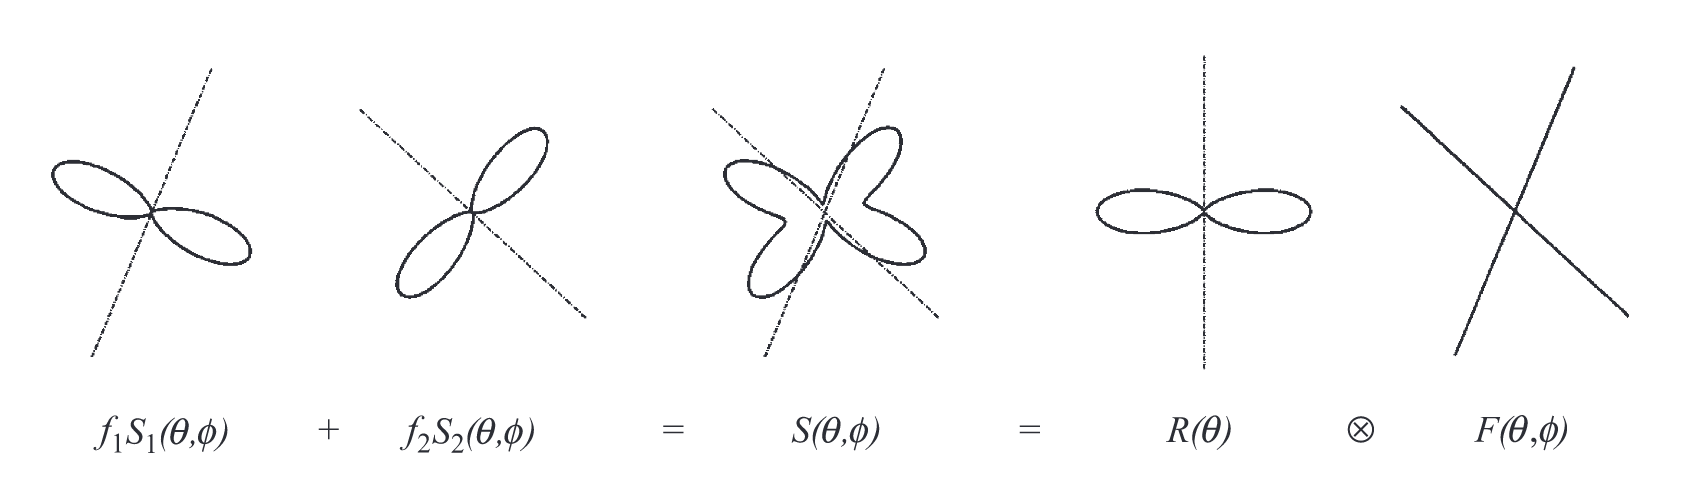
\includegraphics[width= 15cm]{figures/2D.png}
        \caption{In this simple 2D illustration, the voxel contains two fiber populations with distinct orientations
         $(\theta_{1} ,\phi_{1})$ and $(\theta_{2} ,\phi_{2})$, and volume fractions $f1$ and $f2$ ($f1 = f2 = 1/2$ in this case). 
         For each plot, the dotted lines represent the fiber orientation(s) and the continuous line the corresponding signal attenuation. 
         The measured diffusion-weighted signal attenuation $S(\theta, \phi)$ is the sum of each fiber population’s characteristic profile $S_{1}(\theta, \phi) = \hat{A}_{1}R(\theta)$, and $S_{2}(\theta, \phi) = \hat{A}_{2}R(\theta)$, 
         weighted by their respective volume fractions. This can be expressed as a convolution over the unit sphere of an axially symmetric response function R(h), 
         describing the signal attenuation measured for a single fiber population, with a fiber orientation density function $F(\theta ,\phi)$, 
         describing the fiber orientations present in the voxel \cite{tournierDirectEstimationFiber2004}. }
    \label{fig:2dconv}
\end{figure}

\subsection{HARDI}
High angular resolution diffusion imaging (HARDI) is a type of dMRI that measures diffusion signals on a sphere in q-space \cite{consagraOptimizedDiffusionImaging2022}.
During the scanning of high-angular resolution, the signal $S(\theta, \phi)$ is collected in a great number of orientations.
So the white matter structure is estimated by constructing fODF. Spherical deconvolution (SD) is used to estimate fODF in each brain voxel. 
The original diffusion weighted signal is formed from the
various fibre population, and given by spherical convolution of the response functions with the fODF (the apparent density of fibres as a function of orientation) \cite{jeurissenMultitissueConstrainedSpherical2014}. 
If the $R(\theta)$ is known, the fODF can be obtained by the SD of the response function from the measured DW signal inversely.
\subsection{Spherical Deconvolution}
Spherical function is usually represented by a linear combination of spherical harmonics and rotational harmonics. 
The spherical harmonics form a complete orthonormal basis set of functions over the sphere, 
much like the Fourier series forms a complete orthonormal basis over an interval in Cartesian space \cite{tournierDirectEstimationFiber2004}.
Each spherical harmonic contains two main parameters: its order $n$ ($n \geq  0$) and phase factor $m$ ($ -n \leq m \leq n$). 
Increasing order $n$ indicates the higher angular frequency. 

The spherical convolution process is regarded as an action which contains a series of rotation on a function defined over a sphere, which can be related
to the equation \ref{attenuationsignal}. If $\underline{F}^{n}$ is defined to be a vector containing $2n+1$ harmonics in $n$th order 
and $R_{n}$ is the matrix of size $(2n+1)(2n+1)$ representing the $n$th order of rotational harmonics, 
so the $n$th order spherical representation of $S(\theta, \phi)$ can be expressed as:

\begin{gather}\label{sc}  
    S^{n} = R^{n} \underline{F}^{n}
\end{gather}
Therefore, the spherical deconvolution operation can be performed simply by inverting each $R^{n}$ matrix to recover $\underline{F}^{n}$. 

\subsection{Constrained Spherical Deconvolution}
Obtaining the unknown coefficients of fODF through the deconvolution operation on the spherical convolution matrix can be cast as a linear least-squares problem \cite{jeurissenMultitissueConstrainedSpherical2014}.
But this operation can be sensitive to noise and ill-posed. Thus, the constraint SD (CSD) is purposed which performs the SD operation with drastically reduced noise sensitivity, 
allowing reliable fODF estimates on clinically feasible DW-MRI data \cite{tournierRobustDeterminationFibre2007}. CSD performs well in pure WM, while it's prone to produce 
noise in grey matter (GM) and cerebrospinal fluid (CSF) \cite{jeurissenMultitissueConstrainedSpherical2014}. 

So another technique named multi-shell, multi-tissue CSD (MSMT-CSD) is purposed, which assumes that the DW signal arises from the contributions of the three main tissue types found in the brain: WM, GM and CSF \cite{jeurissenMultitissueConstrainedSpherical2014}.
Using MSMT-CSD, the ODF of WM is considered to be anisotropic, while in GM and CSF the ODF is considered to be isotropic and uses an SH series of order 0. 
Some study has shown that compared to single shell single tissue CSD (SSST-CSD), MSMT-CSD can substantially increase the precision of the fODF fibre orientations 
and reduce the presence of spurious fODF peaks in voxels containing GM and/or CSF \cite{jeurissenMultitissueConstrainedSpherical2014}.

\section{Tractography}

Test \autocite{dhollanderFixelbasedAnalysisDiffusion2021}


\section{Fibre Filtering Methods}

\subsection{COMMIT}

\subsubsection{Filtering Theory}

\subsubsection{Existing Problems}

\subsection{SIFT}

\subsubsection{Filtering Theory}

\subsubsection{Filtering Theory}

\section{Deep Learning Based Classification}

\subsection{Multiple Layer P}
\subsection{RNN}





\chapter{Methods}

This chapter introduces the outline of this project, the datasets used in the experiments, the hardware and software information, the detailed 
explanation of the experiment design and the construction of deep learning models.

\section{Projects Outline}
The project was performed in following steps:
\begin{itemize}
    \item Access and preprocess the datasets if necessary.
    \item Apply rCOMMIT experiment on the target datasets
    \item Extract pseudo ground truth from the experiment results.
    \item Construct deep learning models.
    \item Train and tune the models to achieve stable performance.
    \item Compare the results between models.
    \item Compare the results with previous research.
  \end{itemize}

\section{Datasets}
In this project, the preprocessed datasets of six different subjects from the young adult data set of the Human Connectome Project \cite{vanessenWUMinnHumanConnectome2013} are used as raw data.
The tractograms are generated by the authors of \cite{TractSegFastAccurate} with iFOD2 \cite{tournierImprovedProbabilisticStreamlinesa}. 
Ten million streamlines are generated for each subject and the length of streamlines are restricted to be in the range between 40 mm to 250 mm.
The tracking was further constrained by anatomical priors based on the segmentation of different tissue types in the brain \cite{smithAnatomicallyconstrainedTractographyImproved2012}.
And the ten million streamlines cover the whole white matter of each subject. 

\section{Hardware and Software}
Two Nvidia GPUs are used for the training of deep learning models in this project, which respectively are of 4 GB and 11 GB memory. 
The latter GPU is deployed on a platform, Medical Artificial Intelligence Aggregator (MAIA) \cite{MAIA}, which aims to integrate and promote collaborations in the medical field.

COMMIT \cite{daducciCOMMITConvexOptimization2015} is used as the main filtering tool in the experiments. 
SIFT \cite{smithSIFTSphericaldeconvolutionInformed2013} is used in the previous research from which the results are compared in this study.
MRtrix3 \cite{tournierMRtrix3FastFlexible2019} helps visualize the data to check the white matter region is covered by the streamlines. 
The type of raw data is originally in tck file, and a script from ScilPy realizes the conversion between tck and trk files.
Python library Dipy takes care of postprocessing and analysing the tractograms in the training with DL models.
The neural network is built based on TensorFlow, and the monitor of the training process is done with TensorBoard.

\section{Randomized COMMIT (rCOMMIT)}
Finding anatomical ground truth for tractogram has always been a challenge, so there is no ground truth for the filtering method either.
In addition, the results from the existing filtering methods are not consistent. Both problems make the filtering methods less plausible.
To Avoid biases and extract plausible information from the filtering methods, randomized COMMIT is purposed. 
The main idea of this method is to use multiple assessments from COMMIT on the same streamline in different subsets in order to classify streamlines into different groups.
The filtering process can be regarded as a binary classification, since in one time running of COMMIT, the streamline is either accepted or rejected by the filtering method.
The results from multiple times of filtering are seen as votes that are either positive or negative.

Another concern is the bias of the size of the dataset. Usually for a tractogram of 10 million streamlines, around 2\% - 2.5\% streamlines are remained after filtering.
During the filtering, when the remaining streamlines are too small to guarantee the stability of the computation, the filtering method would terminate the process.
To investigate the performance of COMMIT in different sizes, 
multiple subsets are generated from the raw data. From the raw dateset to the smallest dateset, the size of subsets is automatically chosen, by halving
the subset size. And the smallest size is set to be 2.5\% of the input size. Therefore, all the used sizes include $SS= \left \{  1\times 10^7, 5\times 10^6, 2.5\times 10^6, 1.25\times 10^6, 6.25\times 10^5, 5\times 10^5, 2.5\times 10^5 \right \}$ 

Fig \ref{fig:pipe} shows the whole pipeline of rCOMMIT and the pseudo algorithm of the pipeline is shown in \ref{fig:algo}. 
The process of rCOMMIT will be explained more in details with the pseudo algorithm. rCOMMIT will run on all subsets with predefined
size $n \in SS$, and for each $n$ the repetition time $k$ is calculated according to the formula below:
\begin{gather}\label{computek}  
    k = \tau M/n
\end{gather}
$M$ is the original number of streamlines in the tractogram, and $\tau$ is the parameter set in the experiments, 
which indicates the purposed average filtering times by COMMIT for the streamlines. This parameter helps achieve enough votes for classifying streamlines into groups.
For example, with $\tau=5$, the repetition time $k \in \left \{5, 10, 20, 40, 80, 100, 200 \right \}$ for each size in $SS$.
Therefore, with multiple times of filtering, the acceptance rate (AR) of each streamline can be obtained, which is computed below:
\begin{gather}\label{AR}
    AR(s) = \frac{P(s)}{P(s)+ N(s)}
\end{gather}
$AR(s)$ refers to the acceptance rate for the streamline $s$ after receiving all the votes from the experiment in different sizes.
$P(s)$ stands for the positive votes while $N(s)$ are the negative votes.
It's worthy mentioning that each subset is randomly sampled from the raw data. 
Although a target average number of filtering is set, but the number of occurrences of each streamline in the subsets is not ensured, 
which means the numbers of votes for the streamlines can be various.

\begin{figure}[ht]
    \centering
    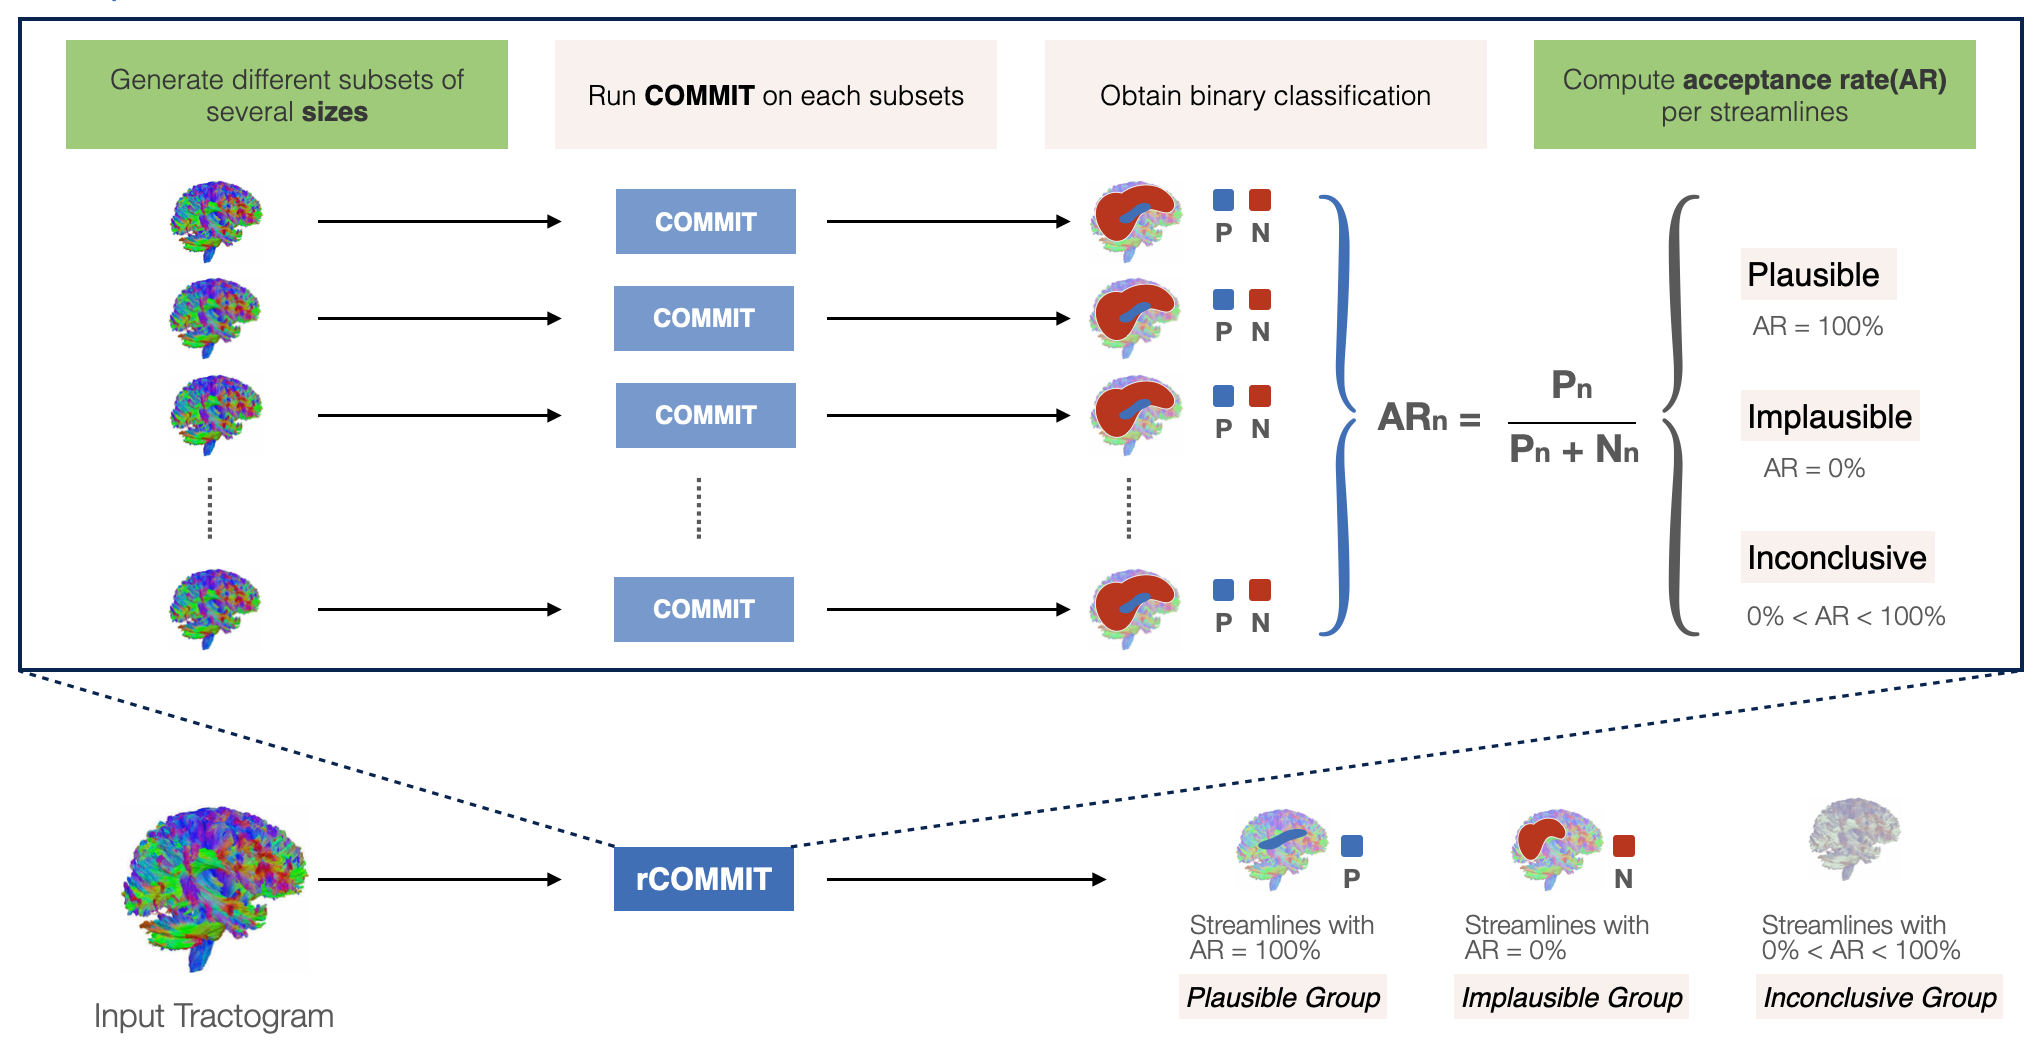
\includegraphics[width= 16cm]{figures/pipe.jpg}
        \caption{The pipeline of rCOMMIT. 
        }
    \label{fig:pipe}
\end{figure}


\begin{algorithm}
    \caption{Pseudocode of rCOMMIT. For the chosen subset size $n$, $k$ random subsets of the tractogram are randomly extracted and filtered with COMMIT to 
    receive the index of the accepted and rejected streamlines $subset_i^P$ and $subset_i^N$. These are used to update the number of votes and compute the acceptance rate in the end.}
    
    \KwIn{
    \begin{tabular}{ll}
    $T = \{t_1, t_2, \ldots, t_{M}\}$ : tractogram,\\
    $SS = \{s_1, s_2, \ldots, s_N\}$ : subset sizes
    \end{tabular}}
    
    \KwOut{
    \begin{tabular}{ll}
    $P = \{p_1, p_2, \ldots, p_M\}$: accepted times,\\
    $N = \{n_1, n_2, \ldots, n_M\}$: rejected times
    \end{tabular}}
    
    \BlankLine
    \BlankLine
    %\Begin{
    Initialize $P$ and $N$ with zeros\\
    \ForAll{$n \in SS$}{
    Initialize $P_n$ and $N_n$ with zeros\\
    $k \gets \tau M/n$\\
    \For{$i \in \{1, \ldots, k\}$}{ 
    $subset_i \gets \{r_1, \ldots,r_n\} \subseteq T$, where $ r_{1, \ldots, n}$ are randomly selected from $T$\\
    $[subset_{i}^P, subset_{i}^N] \gets COMMIT(subset_i)$\\
    $P_n(subset_i^P) \gets P_n(subset_i^P)+1$\\
    $N_n(subset_i^N) \gets N_n(subset_i^N)+1$
    }
    $P= P+P_n$\\
    $N= N+N_n$\\
    
    }
    \label{fig:algo}
    
\end{algorithm}

\section{Pseudo Ground Truth}

After receiving all the votes from the experiments, the acceptance rate can be obtained for almost every streamline.
The pseudo ground truth is based on the acceptance rate of each streamline. This step is based on the very important assumption in this study.
The streamline with higher acceptance rate indicates its better ability to survive from filtering. These streamline are more plausible than those with lower acceptance rate.
To better classify streamlines, strict conditions are made to separate them into three groups:

\begin{enumerate}
    \item Plausible group when $AR = 100\%$
    \item Implausible group when $AR = 0\%$
    \item Inconclusive group when $0\% <AR< 100\%$
  \end{enumerate}

Streamlines being in the plausible group means that they are always accepted by the COMMIT, while in the implausible group the streamlines are always rejected.
These two groups can also be labeled as true and false. Those in the inconclusive group receives inconsistent votes from the COMMIT. 

\section{Deep Learning Streamline Classifier}
rCOMMIT is purposed to extract plausible information from the filtering methods. To further investigate the different properties between groups and the potential
of deep learning methods in filtering field, neural networks classifiers are built and trained on the labeled dataset from the last step.
In the experiment, the classifiers are trained for the binary classifications among three classes and the multi-class tasks.

\subsection{Data Preprocessing}
To make the datasets from different subjects more appropriate for the training process, preprocessing steps are conducted.
Originally, each streamline consists of multiple sampling points and each point has three coordinates. 
First, the streamline coordinates are normalized to the range of -1 and 1 in each dimension using the maximum and minimum values per subject.
However, the sampled points for each streamline are various. Secondly, to standardize the input of each streamline, they are resampled to the same 
number of points. A big number of points from the input streamline might cause expensive computation, while too few points might contain 
inadequate information. So the medium number of streamline points among the training subjects is chosen to be the resampled number, which is 23.
Linear interpolation is used to realize this step. Last, the shape of the streamlines is changed from 3-D into 1-D by flattening the vector. 
The original coordinates are 
In beginning of the preprocessing steps, all the tck files of tractograms are loaded as Numpy arrays, 
so the preprocessing steps can be easily operated with Numpy. 

\subsection{Model Construction}

For the classification tasks, the Convolutional Neural Network (CNN) is widely used. In our study, the classifiers are built on the CNN architecture.
Each classifier contains two 1-D conventional layers with ReLU activation function and the kernel sizes 5 and 3. 
A max-pooling layer with pool size 2 is applied after each of them. Then conventional layers are then followed by the dense layer with a dropout chance.
Last, the dense layer is connected with either one or multiple neurons as output, depending on the classification tasks.

\begin{figure}[ht]
    \centering
    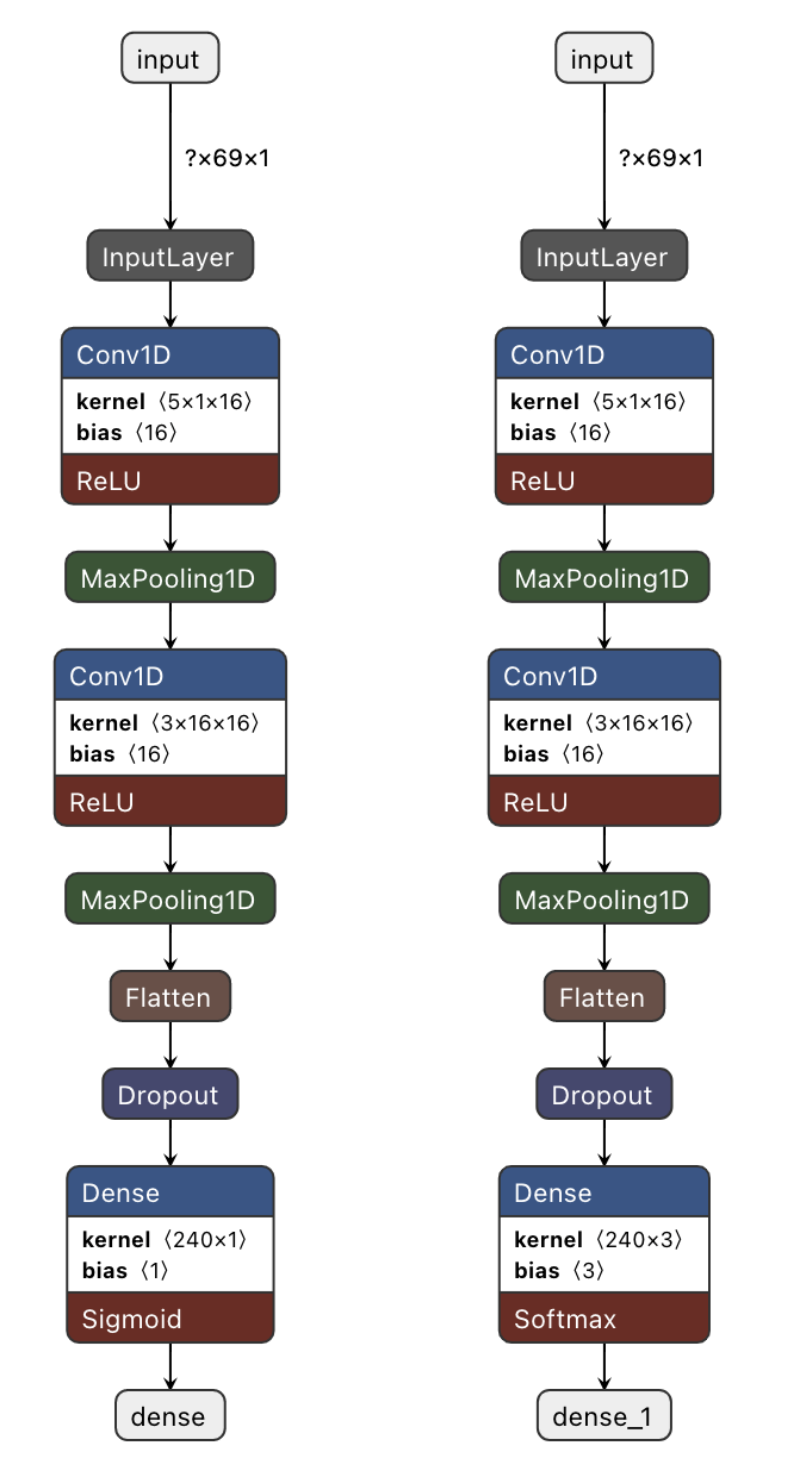
\includegraphics[width= 10cm]{figures/models.png}
        \caption{Architecture of the classifiers. Left: binary classifier. Right: multi-class classifier. 
        The only difference is in the last dense layer. The binary classifier uses one neuron with sigmoid activation, 
        while the multi-class classifier uses multiple output neurons with softmax activation. In our case, the output neurons are 3 for the multi-class classifier.}
    \label{fig:models}
\end{figure}

To do: about RNN model

\subsection{Balance Data Generator}

The data generator is designed to solve the imbalance problem of the dataset. In a binary classification, 
when there is a big imbalance between two classes, for example one class over 90\% and the other one less than 10\%,
the classifier is prone to predict the result to be the bigger class on the normal batch of input. 

In our study, the dataset is mainly based on the filtering method which rejects the majority of the streamlines. 
The disproportion in the dataset is expected. Thus, the data generator is used to over-sample the smaller class for the training and testing.
The batch size is defined to be 60, so it is flexible with two classes and three classes of the input data. 
The epoch size is defined by the larger class and each sub-batch from this class will be seen at least once.
While the sub-batch from the smaller class will be reused and shuffled when it is exhausted during an epoch.










% \chapter{<The work>}

Describe the degree project. What did you actually do? This is the practical description of how the method was applied.

\chapter{Results}

The results will include three parts. 
First, the performance of rCOMMIT will be visualized from different angles. Second, the performance of the models based on the 
pseudo ground truth will be shown. Last, a comparison between the results from COMMIT and SIFT is conducted.

\section{Performance of rCOMMIT}

Fig \ref{fig:heatmap} shows the distribution of AR ranges in different subset sizes on three subjects. 

\begin{figure}[ht]
    \centering
    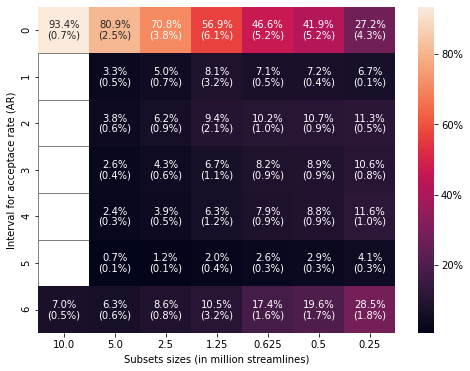
\includegraphics[width= 15cm]{figures/heatmap.png}
        \caption{The 
        }
    \label{fig:heatmap}
\end{figure}

\subsection{Pseudo Ground Truth}

\section{Model Classification}

\section{Comparison Between COMMIT and SIFT}

\subsection{Performance between methods}








Describe the results of the degree project.

\chapter{Discussion}
Tractogram filtering methods like COMMIT exploit the diffusion data and improve the plausibility of 
the streamlines by removing the redundant and wrong streamlines in a way. 
However, COMMIT method is still limited. Delighted by the study on SIFT \cite{hainAssessingStreamlinePlausibility2022}, 
we purpose the rCOMMIT experiment to 
investigate the biases and limitations of COMMIT. Meanwhile, this experiment provides a way 
to extract more plausible streamlines based on filtering methods. 
In addition, the comparison study between COMMIT and SIFT is conducted. 
And neural networks are used to further investigate the characteristics of the streamlines from 
different groups, which show the potential of deep learning in filtering field. 
So the following sections will summarize, compare and explain the results. 
The possible errors and limitations during 
the study are also discussed. Moreover, the future work of this project are discussed.

\section{rCOMMIT}
From the results in results section, COMMIT has shown that the same streamline can be accepted or rejected in different runs, which is 
how the implausible group is defined in the study. This phenomenon indicates that the way COMMIT realizes filtering doesn't depend
on the anatomy of each streamline. And the process of filtering tries to find a subset of streamlines that can improve 
the consistency between tractogram and diffusion data with global optimization approach \cite{hainAssessingStreamlinePlausibility2022}.
Instead of assessing an individual streamline, COMMIT tries to fit with all streamlines as input. 
As shown in the results, with smaller input tractogram, the proportion of accepted streamlines gets higher 
(7.0\% for the whole tractogram vs. 28.5\% for the smallest subset). From the whole tractogram to the smallest subset, the proportion of 
the rejected streamlines decreases from  93.4\% to 27.2\%. 
A possible explanation is that the smaller subsets might contain fewer redundant streamlines, so that the accepted proportion increases
due to the lower base number. 

Also, the ground truth of the anatomy of the streamlines is deficient for most of the tractograms, 
which brings another limitation to the filtering method. For these limitations, rCOMMIT method is designed to give an independent
assessment on each streamline. The independence of the assessments comes from the randomized sampling and the separation between runs.  
Although the ground truth is still lacking for rCOMMIT, the classified streamlines from rCOMMIT are statistically plausible which avoid 
the bias of size compared with COMMIT. 

Besides, the bias on length during the filtering by COMMIT is also confirmed in this study.
From the distribution of the number of streamlines with the respect to the length, it's obvious that 
there is greater variety in the rejected streamlines by rCOMMIT than the accepted group. 
This phenomenon is also found in SIFT that it tends to filter out longer streamlines.
A guess on this problem is that the longer streamlines are prone to give more error during the optimization process
to find the best set of streamlines. To reach the minima, these streamlines are more likely to be filtered. 
However, from the current results, there isn't a very convincing explanation for it. 

\section{Comparison Between rCOMMIT and rSIFT}

Comparing the results from rSIFT with rCOMMIT, we conclude that SIFT method in general is more strict in filtering than COMMIT. From the results, SIFT 
is prone to reject more streamlines when applying both methods on the same tractogram.  
The difference from the filtering theories may explain this. 
Both methods seek for a set of streamlines that could best describe the data. For COMMIT, the data to be reconstructed by the streamlines is measured diffusion data, while 
SIFT aims to associate the streamline densities with FOD lobe integrals, which is a representative of the diffusion data. Besides,
during filtering, SIFT removes streamlines iteratively to better fit the measured data, so that this process is irreversible. And it's 
also possible that the solution reaches local minima instead of a global solution.


From the venn diagrams, there is a big intersection between the implausible groups from rSIFT and rCOMMIT, 
and most of the implausible streamlines from rCOMMIT are also included in by rSIFT. For the plausible 
group, the rSIFT has a smaller group of streamlines. The proportion of the intersection to plausible groups is not 
as big as the proportion of the implausible intersection. Although the theories of filtering differ from each other,
the results of implausible streamlines from both methods are largely overlapping. 
The theories behind these methods may also explain it. The iterative and irreversible removal of streamlines in SIFT filters out more streamlines than COMMIT,
and COMMIT computes the weight for each streamline which represents their contribution to the reconstruction of the diffusion signal. 
The less plausible streamlines may of lower weights, but they can still be in the reconstruction, but these streamlines might be removed by SIFT.


\section{Classification}

Neural networks are exploited for different classification tasks and to show the potential of deep learning methods in filtering.
The binary classifiers trained on the plausible and implausible groups from rCOMMIT obtained an average accuracy of 78\%, which indicates the 
structural differences between these two groups that can be learned by the neural networks. Since the whole process of rCOMMIT is very time-comsuming,
the binary classifiers applied on the unknown subject also shows its ability in distinguishing plausible streamlines from the implausible ones.

The binary classifiers trained on the plausible and implausible intersections between rCOMMIT and rSIFT show the even higher accuracy than
the one trained on the pseudo ground truth from rCOMMIT. As mentioned, compared with their own groups, the proportion of the plausible intersection is not as big as the 
implausible intersection. Because the performance of the classifiers is improved from the new training data, we conclude that within the same
structure of the neural networks and hyperparameters there is greater difference between plausible and implausible intersections.
Since the implausible intersection is very closed to the implausible group from rCOMMIT, the difference mainly comes from the plausible intersection.
Based on this combined information from two methods, we conclude that the overlapping streamlines are likely to survive from filtering and be more plausible.

% (to do) When the classifiers based on the intersection data are applied on the unknown subject, ...  

The binary classifiers are also respectively trained on the plausible non-intersection groups and implausible non-intersection groups from both methods.
We assume that the performance of classifiers can indirectly indicate the difference between the non-intersection parts.
With the same hyperparameters and the structure, 
the mean accuracy of the classifiers trained on the plausible non-intersection groups is higher than the other.
It indicates that it's easier for the same model to learn the difference between the plausible non-intersection groups,
so there might be a greater difference between the plausible streamlines that are chosen by two methods.
However, from the venn diagrams show the difference in the amounts of streamlines in different groups which might
also explain the performance of classifiers. 
Because the implausible non-intersection group from rCOMMIT is rather small compared to the one from rSIFT.
And the proportion between the two plausible non-intersection groups is relatively balanced.
Although during the training the data generator is used to balance the two input classes, there still
might be not enough various streamlines for the model to study. 
In the end, we can't come to any conclusion about the difference in non-intersection groups.


\section{Source of Error}

In the design of rCOMMIT, some drawbacks should be emphasized. The concept of AR helps classify the streamlines, but the 
computation of the AR depends on the base number of runs by COMMIT for each streamline. 
Although in each size level of subsets the streamlines are on average assessed by COMMIT 5 times, some streamlines still get fewer assessments,
which might cause bias to the AR value. One possible solution is to choose the streamlines with 5 times assessments before
generating the pseudo ground truth. It ensures that the ARs are computed with the same denominator, 
but the total number of streamlines from the pseudo ground might differ between subjects.
The second solution is increasing the sizes of subsets in the experiments, which will reduce the impact from the bias but not remove it.
To assess this bias, a distribution of classification results from streamlines with 5 votes can help.




\section{Future Work}

There are several questions remained after this study. The bias on the length of the filtering methods
is found but lack of explanations. Deep learning models can be used to investigate this question indirectly as well.
For example, the accuracy of the classifiers trained on streamlines of different lengths might give some evidences.  
Besides, the plausible groups from both two methods can be an interesting angle to 
study the difference between filtering methods.  

This classifier built in this study shows the potential of DL methods, so it's promising to have applications 
based on DL for filtering in the future. Also, there are some existing ground truths for some tractograms that 
can be used for training. The time and computation of the filtering process can be improved by DL.   

In addition, there is plenty of work can be addressed in improving the accuracy of the networks.
For example, using more information about the structure of the streamlines to the network
and trying different types of neural network are worthy to be studied. Since only the 1-D information of the 
coordinates of sampling points are used in this study, more structural features from the input data might 
help the network learn more about the anatomy of plausible streamlines.

Besides COMMIT and SIFT, there are other filtering methods such as LiFE, SIFT2, COMMIT2 to be investigated.
The difference and similarity between the methods are not very clear. Similar experiments can be conducted and 
more information about filtering methods can help achieve better quality of tractograms for further research.







\chapter{Conclusion}
In this study, we proposed rCOMMIT as a method to study the performance of 
filtering method COMMIT and give assessment on individual streamlines. 
The results from the rCOMMIT shows the biases during the filtering and comfirm the 
biased assessment on individual streamlines. 

Additionally, the pseudo ground truth for the input data is generated with rCOMMIT,
which divides the input streamlines into three groups (plausible, implausible, and inconclusive).
Based on this data, deep learning-based classifiers are trained to distinguish different streamlines.
The classifiers are applied to both binary and multi-classes classification tasks and 
show the potential of deep learning method in filtering. 
It learns the characteristics of different type of streamlines 
and speeds up the filtering process.  

Moreover, with findings from the previous research on SIFT, comparisons between two filtering
methods are conducted. The study shows that SIFT method is stricter in filtering than COMMIT.
And the intersections between two methods improve the performance of classifiers, and reflect the difference
between plausible groups from both methods. 



% \include{content}

\newpage
\addcontentsline{toc}{chapter}{References}
\textbf{If you are using mendeley to manage references, you might have to export them manually in the end as the automatic ways removes the "date accessed" field}
\printbibliography


\newpage
\appendix
\newpage
\etocdepthtag.toc{mtappendix}
\etocsettagdepth{mtchapter}{none}
\etocsettagdepth{mtappendix}{subsection}
\etoctocstyle{1}{Appendix - Contents}
\tableofcontents
\newpage


\chapter{First Appendix}


\chapter{Second Appendix}
This part aims to give background information about this thesis in the field of filtering methods on nerve tracts using data collected by diffusion MRI. 

% \renewcommand{\thesection}{\Alph{section}}
% \renewcommand{\thesubsection}{\Alph{subsection}}

\section{Diffusion Magnetic Resonance Imaging}
\label{sec:dmri}

Diffusion magnetic resonance imaging (dMRI) has led to discoveries of microstructure and connectivity in human brain.
It is the only non-invasive way to 
systematically map white matter tracts in human brain.
dMRI exploits the natural movement of water molecules 
which exists in micro brain tissues. 
This natural movement, as known as Brownian motion, 
is regarded as random motion of molecules. 

The random displacements of molecules 
resulting from thermal agitation (Brownian motion) 
obey a statistical law established by Einstein in 1905 \cite*{lebihanLookingFunctionalArchitecture2003}.
Diffusion refers to this phenomenon.
And distance of movements could be described by diffusion coefficient.
If molecules are in a free space, the displacements will obey Gaussian distribution
during a given time period. This kind of diffusion can be viewed as isotropic diffusion.

However, not all the molecules are free inside brain. As it shows in Fig. \ref{fig:brownian},
some of them are constraint inside cells, so their displacements are limited by the size of cells. 
Some other molecules are in a narrow space with obstacles, which only allows molecules
to move along a pathway. Displacements are constraint under this situation.
Molecules are far from "free", so the displacements will not fit in standard Gaussian distribution anymore.
This kind of restricted diffusion is known as anisotropic diffusion.
These phenomena can be captured by diffusion tensor with dMRI, which indirectly reveal the microstructure of brain tissue.
This ability of dMRI is particularly effective for studying the connectivity of the brain,
as it permits to noninvasively estimate the major neuronal pathways in the white matter (WM) 
by means of the so called tractography (also known as fiber-tracking) \cite*{daducciCOMMITConvexOptimization2015}.

\begin{figure}[ht]
    \centering
    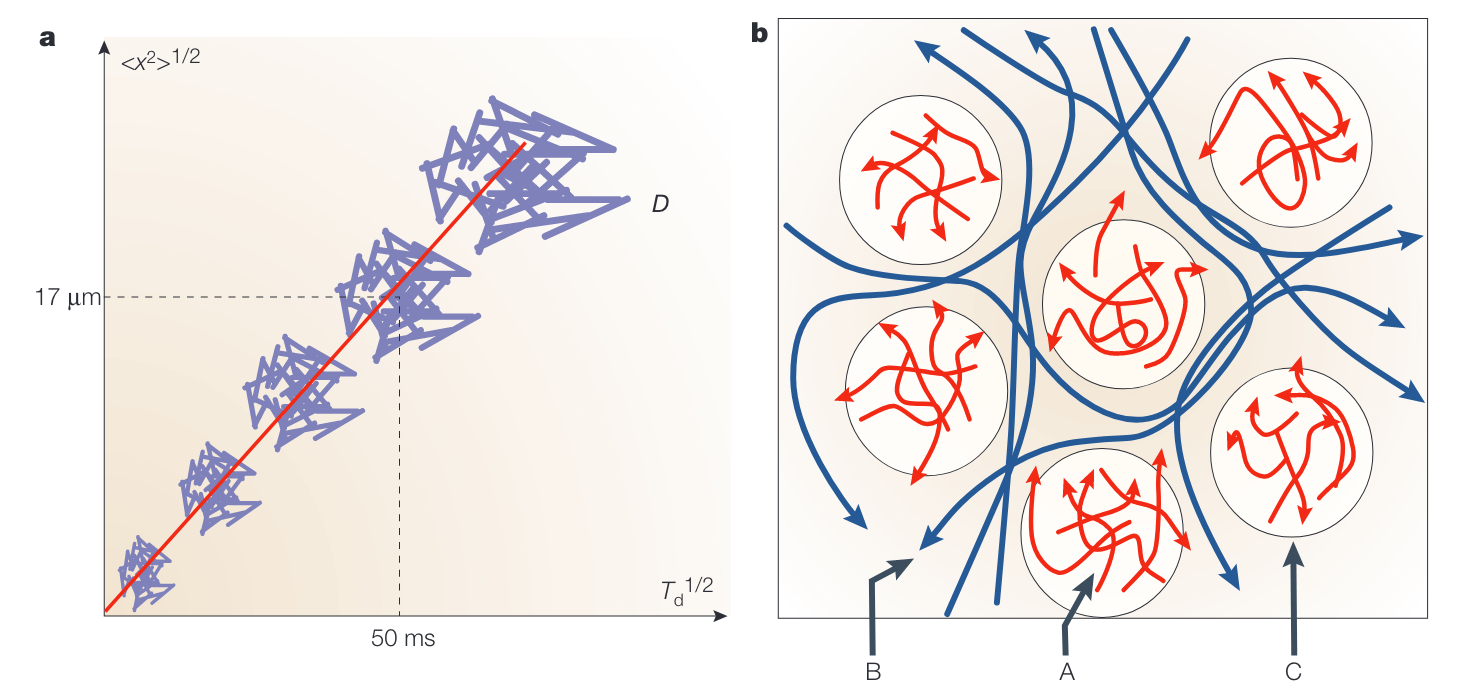
\includegraphics[width= 12cm]{figures/brownian_motion.png}
        \caption{Fig.\textbf{a} shows the relationship among diffusion time, diffusion coefficient and displacement variance.
        ${T_d}$ is the time for molecules to diffuse. $D$ is diffusion coefficient, 
        and <${x^2}$> is the variance of the molecular displacement along that dimension. 
        For water at brain temperature, $68\%$ of molecules have moved within a sphere of $17 \mu s$ diameter in $50 ms$.
        Fig.\textbf{b} mimics biological tissues. Displacements could be constraint in a closed space (A).
        Diffusion might also be hindered by obstacles that result in tortuous pathways (B).
        Exchange between compartments also slows down molecular displacements (C) \cite*{lebihanLookingFunctionalArchitecture2003}.
        }
    \label{fig:brownian}
\end{figure}


\section{Tractography}
\subsection{Diffusion Modeling}

Diffusion data from dMRI will be used to estimate fiber orientations of each voxel. 
This section would introduce some prominent methods and models in this field.

First, standard tensor model introduced by Basser \cite*{Qof40e4TmpElsevier} is the basic model to estimate orientations.
Diffusion tensor in 3D space can be mathematically modeled by a 3 x 3 matrix, which can be written as below. \ref*{tensor_matrix} 
It is a symmetrical, positive tensor consisting of 6 unique parameters. 
Inside $D$, diagonal elements represent diffusion in $x$, $y$ and $z$ coordinates, 
and off-diagonal elements represent correlation of diffusion in two coordinates. 
Diffusion tensor is symmetrical, so it indicates $D_{ij}$ = $D_{ji}$.
Six parameters are enough to build 3 x 3 tensor matrix. 
\begin{gather}\label{tensor_matrix}
    D = 
    \begin{pmatrix}
        D_{11} & D_{12} & D_{13} \\
        D_{21} & D_{22} & D_{23} \\
        D_{31} & D_{32} & D_{33} 
    \end{pmatrix}
\end{gather}

In figure \ref*{fig:DTI}, diffusion tensor imaging(DTI) shows isotropic tensor anisotropic tensor in 
both free space and constraint space. 
$\lambda 1$, $\lambda 2$ and $\lambda 3$ in the tensor model are eigenvalues of diffusion matrix.
Besides, the matrix has three eigenvectors as well. With eigenvalues and eigenvector, the length of diffusion 
and the coordinates of diffusion tensor can be interpreted.

\begin{figure}[ht]
    \centering
    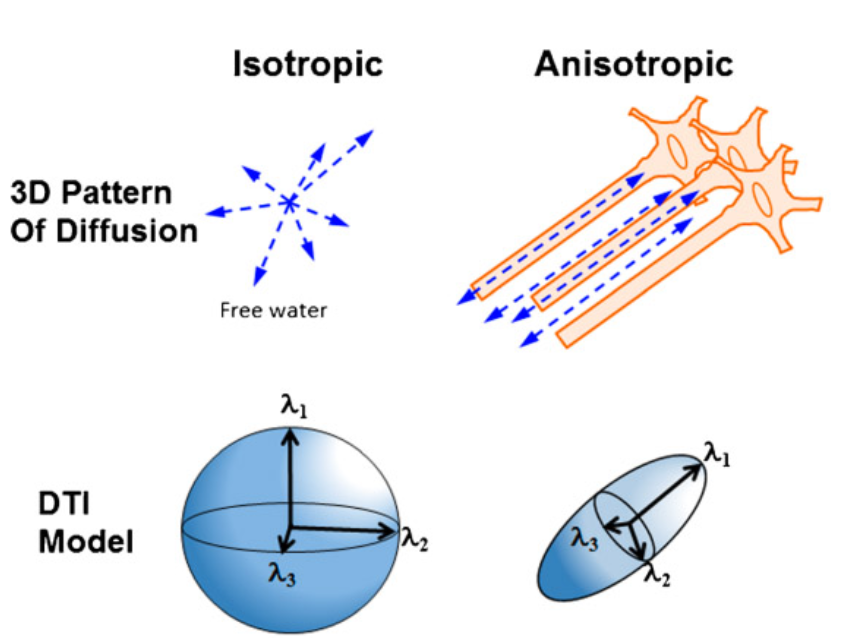
\includegraphics[width= 10cm]{figures/DTI.png}
        \caption{An example showing 3D pattern of diffusion in both free space and constraint space. 
        Second row shows diffusion tensor imaging(DTI) of the according tensor model. 
        $\lambda 1$, $\lambda 2$ and $\lambda 3$ in the tensor model are eigenvalues of diffusion matrix.}
    \label{fig:DTI}
\end{figure}

One major flaw of this model is the inability to represent multiple fiber orientations in a voxel, which can occur due to fiber kissing or crossing \cite*{tournierDirectEstimationFiber2004}.
Besides, there are more pre-defined models including two-tensor model \cite*[]{qaziResolvingCrossingsCorticospinal2009}, ball-and-sticks model \cite*[]{behrensCharacterizationPropagationUncertainty2003}
and neurite orientation dispersion and density imaging (NODDI) model \cite*[]{zhangNODDIPracticalVivo2012}. 
The advantages of these models is that pre-defined patterns in estimating orientations require fewer diffusion sampling directions from dMRI data. 
But when meeting more complex cases such as pathologic data, the results from pre-defined models can't be ensured.

Different from using models, some methods compute the orientational distribution of a voxel. 
Orientation Distribution Functions (ODFs) are the histograms of distribution of diffusion at different dimension. 
Peak values from ODFs can be chosen as orientations during fiber tracking. Methods exploit distribution are flexible with complex condition.
In figure \ref*{fig:odf}, it shows an example of ODF from a voxel computing from samples of multiple directions in dMRI acquisition.

\begin{figure}[ht]
    \centering
    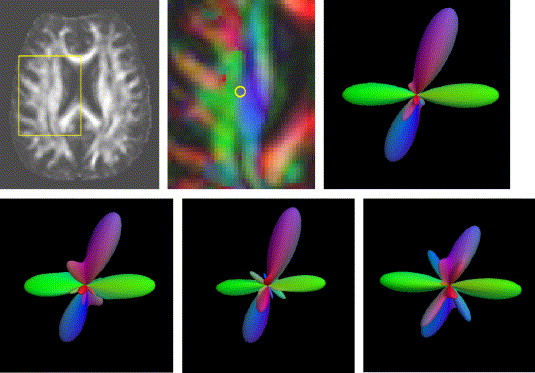
\includegraphics[width= 12cm]{figures/odf.jpg}
        \caption{Fiber ODFs reconstructed from the in vivo data for a voxel.
          Top left: an axial fractional anisotropy(FA) map just below the centrum semiovale. 
          Top middle: a magnified section of the FA map, colored according to the anatomic direction of the major eigenvector of the diffusion tensor 
          (red: left–right, green: anterior–posterior, blue: inferior–superior). 
          Top right: the fiber ODF reconstructed from the highlighted voxel, 
          displayed as a sagittal projection to highlight the presence of the two distinct fiber orientations. 
          Bottom row: fiber ODFs for the same voxel reconstructed using each of the individual 60-direction data sets from data acquisition.
          Note that any negative lobes in the fiber ODF have been discarded. \cite*[]{tournierDirectEstimationFiber2004}
        }
    \label{fig:odf}
\end{figure}

Two types modeling methods mentioned above can be viewed as model-based method and model-free method. 
Spherical deconvolution methods combine both of them. These methods estimate the fiber orientation distribution directly from high angular resolution diffusion-weighted MR data without prior assumptions \cite*[]{tournierDirectEstimationFiber2004}.
On the one hand, these methods also computes ODFs as model-free methods. 

Different from the other two methods, the prior assumption of spherical deconvolution
is that all white matter fiber bundles in the brain share identical diffusion characteristics,
thus implicitly assigning any differences in diffusion anisotropy to partial volume effects \cite*[]{tournierDirectEstimationFiber2004}.
To be specific, the diffusion model in spherical deconvolution comes from selected white matter.
Kernels extracted from diffusion model are called \textit{response functions} and are used to convolve with ODFs.
The results are called fiber orientation distribution (FOD).
Some research indicates that FOD tractography has a better resolving power than DTI and diffusion ODF methods, making it ideal for delineating fibers crossing at a sharp angle \cite*[]{yehTractographyMethodsFindings2021}.
Moreover, all these methods are rather recent, so more studies and validations are needed.

\subsection{Fiber Tracking Methods}

The fiber tracking strategies can be mainly divided into deterministic, probabilistic, and global geometric techniques \cite*[]{ozarslanAnisotropyFieldsScales2021}.
In this paper, we would mainly introduce streamline tracking, a deterministic technique, that is most commonly used algorithm for tractography.

With local data available in the neighborhood of each voxel, fiber tracking can be viewed as solving an \textit{ordinary differential equation} (ODE), 
and the targeted track trajectory is the unknown function to be estimated \cite*{daducciCOMMITConvexOptimization2015}\cite*{yehTractographyMethodsFindings2021}.
The goal of the first-order ODE problem is to numerically estimate an unknown function using both its first derivatives and an initial value of the function \cite*[]{yehTractographyMethodsFindings2021}.
In streamline tracking, the initial value would be the starting point of the trajectory, while the diffusion field is used to interpret derivatives.
Usually the initial values are defined manually. For example, a deterministic algorithms Fiber Assigned by Continuous Tracking (FACT), 
a starting point in gray matter is chosen to be along the biggest main eigenvector of the adjacent voxels. 
% \cite{}
This propagating process from starting point is repeated by integrating in diffusion field at each position until any of termination criteria are met. These criteria include
meeting the boundary of masks and maximum turning angle. 

In figure \ref*{fig:tracking}, the first scenario shows how to use Euler method in calculating fiber trajectory. 
This method also starts with pre-defined points, as known as seeds, and propagates in two opposite directions. At each voxel, the spatial 
information of next voxel is determined by the present voxel and its derivative, 
which can be viewed as $f(t_{i+1}) = f(t_{i}) + f'(t_{i})\Delta s$. And $\Delta s$ here is the step size in propagation.
After propagation on every given seed, all streamlines are finally generated.
The set of obtained streamlines is usually referred to as a tractogram

\begin{figure}[ht]
    \centering
    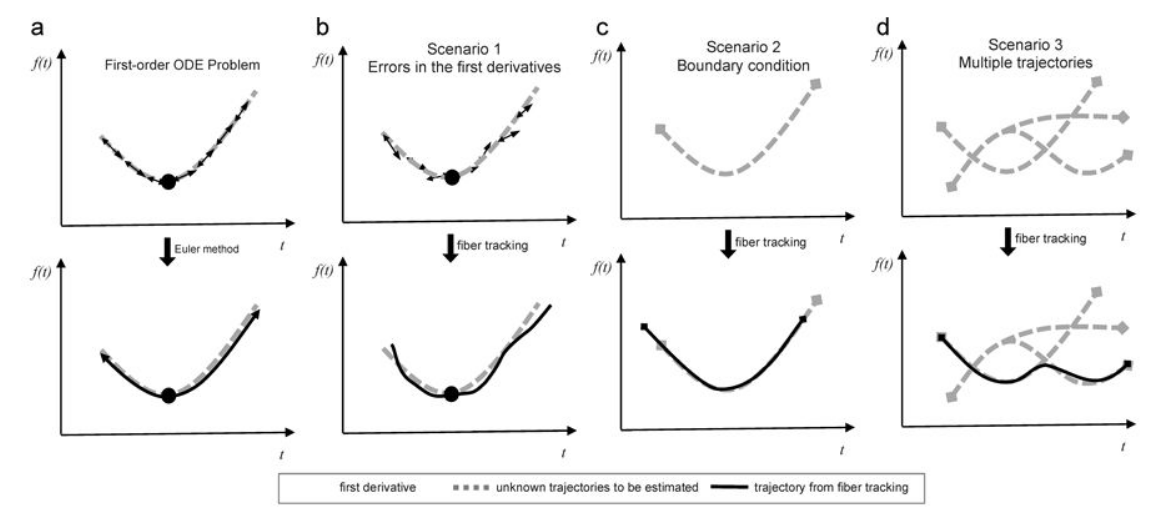
\includegraphics[width= 13cm]{figures/tracking.png}
        \caption{Fiber tracking involves a numerical procedure to solve a first-order ordinary differential equation (ODE) whose parameters are specified by a starting location (i.e., the seeding point, black circle) 
        and by the first derivative of a function (i.e., the resolved fiber orientation, arrows) at each voxel. 
        The trajectory can then be calculated using the Euler method. 
        However, the conventional ODE problem only considers numerical error due to finite step size and does not consider other error scenarios in fiber tracking. 
        The first scenario that raises challenges for standard fiber tracking involves errors in the estimation of first derivatives, 
        which can cause substantial deviation of trajectories from their ground truth. 
        The second challenging scenario involves the boundary condition. Specifically, white matter tracts have termination locations, and fiber tracking may terminate at the wrong location, 
        leading to a premature termination or an overshoot.
        The third challenging scenario involves the coexistence of multiple trajectories at the same voxel location. 
        Inappropriately connecting unrelated trajectories may lead to incorrect streamline routing and spurious tracks. \cite*[]{yehTractographyMethodsFindings2021}
        }
    \label{fig:tracking}
\end{figure}

However, fiber tracking methods suffer from errors. As it shows in the scenario 1 in figure \ref*{fig:tracking},
sometimes local angles can't match properly, which may due to limitation in diffusion modeling or artifact in data acquisition.
Scenario 2 shows the problem with termination criteria. In scenario 3, when multiple trajectories locate in the same space,
it adds difficulty to fiber tracking. Sometimes the tracking method chooses a wrong direction and connects to another nearby fiber.
It is common error when the voxel has complex diffusion.

\subsection{Tractogram Filtering}

Despite the advances in tractography methods, the anatomical accuracy of tractography has not dramatically improved in recent years \cite*[]{schillingLimitsAnatomicalAccuracy2019}.
First, tractography techniques are mainly based on mathematical computation. Not many anatomical requisites have been applied
to it. And we have discussed some limitations in both diffusion modeling and tractography techniques, which remain uncertainty.
Moreover, in the analysis of brain connectivity realized by dMRI, high specificity has been a challenge to tractography.
This refers to the false positives in tractograms.
Several recent studies have unveiled that state-of-the-art methods to construct tractograms suffer both from false positives (FP), 
i.e., streamlines that are not related to anatomical structures \cite*[]{maier-heinChallengeMappingHuman2017}.
The false positive streamlines create bias in any connectivity analysis since non-existent structures are mixed with real ones \cite*[]{gleichgerrchtDeepLearningApplied2018}. 
To reduce the influence of this bias, some methods are used to improve the tractogram quality. 
This section briefly summaries four main methods in tractogram filtering:
\textit{explainability of the diffusion signal, inclusion and exclusion of regions of interest, streamline geometry and shape and streamline similarity and clustering.} 


\subsubsection{Explainability of the diffusion signal}

A tractogram is based on the diffusion signal from dMRI. 
Therefore, synthetic dMRI generated back from a tractogram should be similar to raw data.
The idea of this method is to find a subset of the streamlines that best describes the input dMRI data. 
This method requires dMRI data and a whole tractogram as inputs.

The Convex Optimization Modeling for Microstructure Informed Tractography (COMMIT) \cite*[]{daducciCOMMITConvexOptimization2015} and LiFE \cite*[]{pestilliEvaluationStatisticalInference2014}, 
describe this filtering method in a mathematical way. 
In equation \ref*{explaindiffusion}, $y$ is the vector with the input diffusion signals. 
$A(T)$ is the formula to synthesize the diffusion data from the streamlines of tractogram $T$, 
while $x$ is the vector with weight for each streamline. And $\eta$ is the acquisition noise. 
Since the $x$ that represents the weights of streamlines will not be negative, 
it is possible to find a minimum for $\eta$. 

\begin{gather}\label{explaindiffusion}  
    y = A(T)x + \eta\\
    \underset{x>=0}{argmin}||A(T)x-y||_{2}^{2}
\end{gather}



SIFT \cite*{smithSIFTSphericaldeconvolutionInformed2013} and SIFT2 \cite*{smithSIFT2EnablingDense2015} share the same idea of explainability,
but their purpose is not to synthesize raw dMRI data with the best combination of streamlines. 
Instead, they focus on removing the less relevant streamlines for better fitting raw data.
Specificlly, the algorithms remove streamlines iteratively to find the minimal sets of streamlines.
However, the removed streamlines won't come back to the results, which means this method can run into local minima.
Another difference of SIFT from the other methods is that it only generate binary labels of streamlines.


Based on this method, a common problem with some mentioned tools is inconsistency in results. 
In practice, results on the same tractogram from either SIFT or COMMIT
sometimes won't be consistent from multiple runtime. 
Same for the same streamline, these tools can't be sure of having the same labels or weight values every time.
The size of tractograms and the length of streamlines can be bias factors to this type of method.

The main purpose of this report is to improve plausibility of the results from COMMIT, 
as well as analyze the impact from multiple biases.


\subsubsection{Inclusion and exclusion of regions of interest}
This method respects the anatomy of the brain by using segmentation masks to filter false positive streamlines. 
To achieve an anatomically correct segmentation, registration to standard atlas is required. 
Streamlines totally outside masks or against anatomical atlas will be filtered. 
The intrinsic problem with this method is about inaccurate registration.
For example, shape of neural fibers changes when a tumour continuously growing inside the brain. 
Using these methods to register dMRI data of a pathologic brain to a standard healthy atlas is not reasonable.
Moreover, registration of brain brings uncertainty as well.


\subsubsection{Streamline geometry and shape}

This method exploits geometrical properties of streamlines.
Shape features of streamlines include the maximum local curvature, the maximum and minimum length of streamlines and so on. 
Some characteristics not existing in real brain should be avoided, such as an unrealistic loop of streamlines. 

Deep learning methods have taken geometry of streamlines as criteria, such as TRAFIC \cite*{lamTRAFICFiberTract2018}. 
It trains a neural network with features such as distances to five landmarks, curvature and torsion per tract as features for filtering \cite*{lamTRAFICFiberTract2018}.

\subsubsection{Streamline similarity and clustering}

The number of streamlines can easily reach 10 million before analysis. 
This method helps cluster streamlines in bundles before analysis. 
From the view of analysis, small bundles that contribute little to the connectivity analysis can be filtered. 
So the only requirement for using standard clustering algorithms for streamline clustering 
is to define a distance metric between streamlines \cite*[]{ozarslanAnisotropyFieldsScales2021}.
The method seems to be very straightforward, but it's not easy to find the best distance for all streamlines.


\section{Deep Learning Methods}
\subsection{Multilayer Perceptron (MLP)}

\section{Structural Connectivity Networks}

% \subsection{Brain connectivity}
% As we know, brain is the main processor of human. 
% It's a complex organ in charges of sense, motor motion, emotion, vision, breathing and
% every process happening to human body.
% Inside brain, neuron is the key unit that support brain to execute all the processes.
% A neuron has three main parts: dendrites, an axon, and a cell body (soma).

\subsection{Brain Connectivity Creation Pipeline}



\newpage
% This is the last page of the document
\thispagestyle{empty}
\AddToShipoutPictureBG*{%]
    \AtPageLowerLeft{%
        
\includegraphics[width=1.0\paperwidth]{setup/img/kth-footer.png}
    }%
}

\PlaceText{20mm}{282mm}{\color{white}\fontsize{12}{0}\sffamily www.kth.se }


\end{document}
